% Provenance (never printed): see sources/outline_sources.md (Year 3:
% facies analysis, depositional models, Walther's law, well logs). Brief:
% sources/book5/BRIEFS.md, ch. 17. Curves from figdata/bachelor-3/well_logs.py
% (unit tops from figdata/shared/region.py). Exercise and problem values in
% the Book 5 scratch calculator calc/ch17.py. The well Varden-2, its logs and
% the channel architecture of its sandstone are invented.
\chapter{Model fasies}\label{ch:b3:facies-models}

Inti dari sumur sedalam satu kilometer: satu meter pasir kasar dengan
perlapisan silang yang bertumpu pada bidang dasar tajam, menghalus ke atas menjadi lanau
berjejak akar, lalu pasir lagi di atas bidang dasar tajam lain. Ahli geologi membaca
sebuah sungai yang berkelok-kelok melintasi dataronya, meski kini tak ada sungai di sana. Pembacaan itu
bertumpu pada dua alat: seperangkat model, masing-masing merupakan ringkasan dari banyak
contoh modern dan purba untuk satu lingkungan, dan sebuah hukum yang mengubah urutan vertikal
lapisan menjadi peta lingkungan-lingkungan yang bertetangga.

\begin{recall}
Fasies sedimen, lingkungan pengendapan, bentuk dasar, perlapisan silang,
ketiga jenis delta, arus turbidit, turbidit, dan lapisan bergradasi ada di
volume Tahun 1, pada bab tentang sedimen klastik dan
lingkungannya; pabrik karbonat, terumbu, dan platform karbonat ada di
bab tentang sedimen karbonat, silika, dan evaporit; log lubang bor dan
korelasinya dalam bab tentang penampang melintang. Porositas dan
permeabilitas ada di volume-volume sekolah. \omterm{def:b3:sequence-stratigraphy:parasequence}{Parasekuen}, \omterm{def:b3:sequence-stratigraphy:parasequence}{permukaan genang}, dan
\omterm{def:b3:sequence-stratigraphy:tract}{traktus sistem} ada di Bab~\ref{ch:b3:sequence-stratigraphy}. Gelombang di
laut dalam, yang geraknya memudar seiring kedalaman, ada di buku fisika.
\end{recall}

\section{Fasies, suksesi, dan hukum Walther}\label{sec:b3:facies-models:walther}

Fasies sedimen dideskripsikan dari apa yang tampak pada inti bor atau
tebing: ukuran butir, pemilahan, struktur, fosil, warna. Satu fasies
jarang bersifat diagnostik: pasir perlapisan silang terbentuk di sungai, di pantai, di
saluran pasang surut, dan di gurun. Yang mengidentifikasi suatu lingkungan
adalah fasies lain yang menyertainya dan urutan saat fasies saling menyusul.

\begin{definition}[Asosiasi fasies dan suksesi fasies]\label{def:b3:facies-models:association}
Yang disebut \emph{asosiasi fasies}\index{asosiasi fasies} adalah kelompok fasies
yang muncul bersama dan diendapkan dalam satu lingkungan, misalnya pasir saluran,
lanau tanggul alam, dan lumpur dataran banjir berakar. Yang disebut \emph{suksesi
fasies}\index{suksesi fasies} adalah urutan vertikal fasies yang
beberapa sifat berubah bertahap ke atas; dalam \emph{suksesi menghalus
ke atas}\index{suksesi menghalus ke atas} ukuran butir turun ke atas,
sedangkan dalam \emph{suksesi mengasar ke atas}\index{suksesi mengasar ke atas}
ukurannya bertambah ke atas.
\end{definition}

\begin{definition}[Model fasies]\label{def:b3:facies-models:model}
Yang disebut \emph{model fasies}\index{model fasies} adalah ringkasan umum dari suatu
lingkungan pengendapan, disarikan dari banyak contoh modern dan purba: fasies
yang dihasilkannya, geometrinya, hubungan lateralnya, serta
suksesi yang dibentuknya. Model ini berfungsi sebagai norma pembanding untuk
contoh baru, panduan pengamatan lanjutan, peramal dalam situasi baru, dan dasar
untuk menafsirkan lingkungan pengendapan.
\end{definition}

Jembatan antara sisi lateral dan vertikal berupa sebuah hukum. Pada setiap saat,
lingkungan yang bertetangga berdampingan: gisik di samping \omterm{def:b3:facies-models:shoreface}{muka pantai},
\omterm{def:b3:facies-models:shoreface}{muka pantai} di samping lumpur lepas pantai. Ketika garis pantai bergerak,
setiap lingkungan berada di atas tetangganya.

\begin{theorem}[Hukum Walther]\label{thm:b3:facies-models:walther}
Dalam suksesi selaras, tanpa jeda pengendapan yang berarti atau
permukaan erosi, fasies yang terletak langsung di atas satu sama lain diendapkan
dalam lingkungan yang pada waktu itu berdampingan.
\end{theorem}

\begin{proof}
Tinjau jalur-jalur lingkungan, masing-masing berupa jalur sejajar garis pantai, yang
bermigrasi bersama melintasi cekungan selama dasar cekungan turun atau permukaan
laut naik. Di suatu tempat tetap, jalur-jalur itu melintas satu demi satu, sesuai urutan
letak mereka berdampingan, dan masing-masing meninggalkan endapannya di atas
endapan jalur yang mendahuluinya. Jika pengendapan menerus, maka urutan
vertikal endapan karena itu sama dengan urutan lateral jalur-jalurnya.
Jeda atau permukaan erosi memutus argumen ini: jalur-jalur yang lewat
selama celah itu tidak meninggalkan apa-apa, atau endapannya tersapu, sehingga fasies dari
lingkungan yang tidak bersebelahan saling bersentuhan.
\end{proof}

\begin{omfigure}
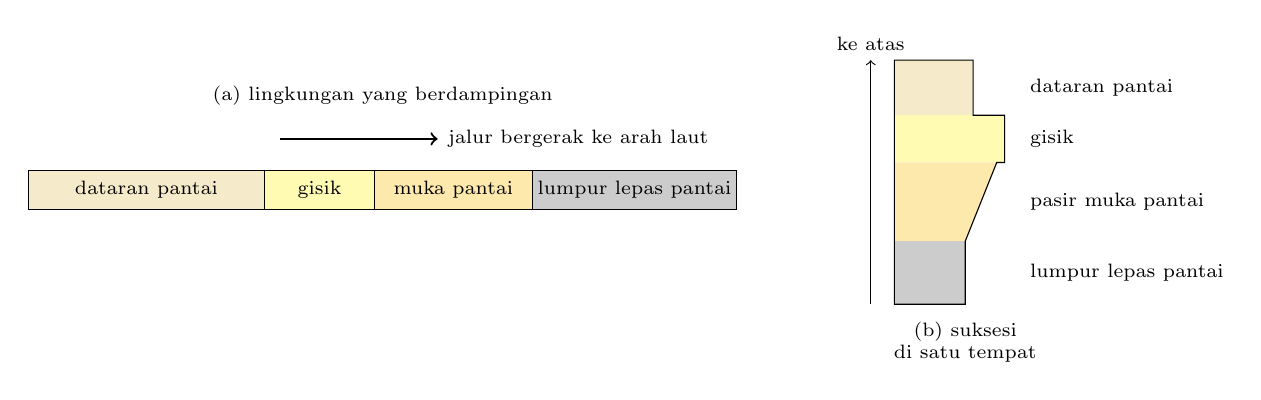
\begin{tikzpicture}[font=\scriptsize, x=1cm, y=1cm]
% environments side by side, with a shoreline that moves seaward
\fill[yellow!35!brown!25] (0,0) rectangle (3,0.5);
\fill[yellow!30] (3,0) rectangle (4.4,0.5);
\fill[yellow!50!orange!30] (4.4,0) rectangle (6.4,0.5);
\fill[black!20] (6.4,0) rectangle (9,0.5);
\draw (0,0) rectangle (9,0.5);
\foreach \x in {3,4.4,6.4} {\draw (\x,0) -- (\x,0.5);}
\node at (1.5,0.25) {dataran pantai};
\node at (3.7,0.25) {gisik};
\node at (5.4,0.25) {muka pantai};
\node at (7.7,0.25) {lumpur lepas pantai};
\draw[->, thick] (3.2,0.9) -- (5.2,0.9) node[right] {jalur bergerak ke arah laut};
\node[anchor=south] at (4.5,1.2) {(a) lingkungan yang berdampingan};
% vertical succession at a place
\begin{scope}[xshift=11cm, yshift=-1.2cm]
\fill[black!20] (0,0) rectangle (0.9,0.8);
\fill[yellow!50!orange!30] (0,0.8) -- (0.9,0.8) -- (1.3,1.8) -- (0,1.8) -- cycle;
\fill[yellow!30] (0,1.8) rectangle (1.4,2.4);
\fill[yellow!35!brown!25] (0,2.4) rectangle (1.0,3.1);
\draw (0,0) -- (0.9,0) -- (0.9,0.8) -- (1.3,1.8) -- (1.4,1.8) -- (1.4,2.4) -- (1.0,2.4) -- (1.0,3.1) -- (0,3.1) -- cycle;
\node[anchor=west] at (1.6,0.4) {lumpur lepas pantai};
\node[anchor=west] at (1.6,1.3) {pasir muka pantai};
\node[anchor=west] at (1.6,2.1) {gisik};
\node[anchor=west] at (1.6,2.75) {dataran pantai};
\draw[->] (-0.3,0) -- (-0.3,3.1) node[above] {ke atas};
\node[anchor=north, align=center] at (0.9,-0.1) {(b) suksesi\\ di satu tempat};
\end{scope}
\end{tikzpicture}

\par\smallskip{\small Hukum Walther. (a) Lingkungan-lingkungan terletak berdampingan sepanjang
suatu profil; (b) ketika sabuk-sabuk bergerak ke arah laut, satu tempat menerima lumpur lepas pantai,
lalu pasir \omterm{def:b3:facies-models:shoreface}{muka pantai}, pasir gisik, dan endapan dataran pantai: \omterm{def:b3:facies-models:association}{suksesi
mengasar ke atas} dengan urutan sabuk-sabuk tersebut (lebar pada log
menunjukkan butir yang lebih kasar).}\label{fig:b3:facies-models:walther}
\end{omfigure}

Hukum ini berlaku dua arah. Regresi menumpuk sabuk-sabuk menurut urutan ke arah laut
ke atas, sedangkan transgresi menumpuknya dalam urutan terbalik; dan suksesi vertikal yang dibaca
pada inti bor memberikan peta lingkungan di sekitarnya pada saat itu. Hukum ini gagal
persis di tempat Bab~\ref{ch:b3:sequence-stratigraphy} menempatkan permukaan-permukaan kuncinya:
yakni di seberang \omterm{def:b3:sequence-stratigraphy:sequence}{batas sekuen}, tempat pemaparan dan erosi membawa pasir sungai ke atas
lumpur paparan, dan di seberang \omterm{def:b3:sequence-stratigraphy:parasequence}{permukaan genang}, tempat lumpur lepas pantai berada langsung di atas
dataran pantai.

\section{Sungai}\label{sec:b3:facies-models:rivers}

\begin{definition}[Sungai teranyam dan sungai bermeander]\label{def:b3:facies-models:rivers}
Yang disebut \emph{sungai teranyam}\index{sungai teranyam} mengalir melalui beberapa
alur dangkal yang bercabang dan menyatu kembali di sekitar gosong, pada dataran curam
dengan beban kasar yang melimpah dan debit yang berubah-ubah. Yang disebut \emph{sungai bermeander}\index{sungai bermeander}
mengalir dalam satu alur berkelok pada dataran yang lebih landai, dengan membawa lebih banyak
sedimen halus; sungai ini berpindah dengan mengikis tebing luar setiap tikungan dan
mengendapkan material pada tebing dalamnya. Endapan pada tebing dalam disebut \emph{gosong
tepi}\index{gosong tepi}. \emph{Avulsi}\index{avulsi} adalah peninggalan
suatu alur demi jalur baru melintasi dataran banjir, biasanya setelah banjir
menjebol tanggul alam.
\end{definition}

\omterm{def:b3:facies-models:rivers}{Gosong tepi} tumbuh ke samping seiring tikungan berpindah, sehingga di suatu tempat ia merekam
penampang melintang alur dari bawah ke atas: lag dari klastika paling kasar di atas
dasar erosional, pasir berlapis silang dari gumuk pasir di alur dalam
, pasir lebih halus dengan riak dari puncak dangkal gosong, lalu
lanau dan lumpur dataran banjir dengan akar dan tanah. Menurut hukum Walther, \omterm{def:b3:facies-models:association}{suksesi
menghalus ke atas} ini, yang tebalnya beberapa meter, sama dengan
kedalaman alur. \omterm{def:b3:facies-models:rivers}{Sungai teranyam} meninggalkan lembaran pasir dan kerikil berlapis silang yang bertumpuk
dan kerikil dengan sedikit lumpur, yang ukuran butirnya hampir tidak berubah ke atas;
fraksi halusnya terbawa pergi. \omterm{def:b3:facies-models:rivers}{Avulsi} memindahkan sabuk alur melintasi dataran, sehingga
endapan alur bertumpuk secara acak di antara lumpur dataran banjir, dipisahkan oleh dasar
erosional yang tajam.

\begin{omfigure}
\begin{tikzpicture}[font=\scriptsize, x=1cm, y=1cm]
% (a) braided plan
\begin{scope}
\fill[yellow!35!brown!20] (0,0) rectangle (4.6,2.4);
\draw[omDef!60, line width=1.6pt] (0,1.2) .. controls (0.8,1.6) and (1.4,0.6) .. (2.3,1.0) .. controls (3.0,1.3) and (3.6,0.7) .. (4.6,1.0);
\draw[omDef!60, line width=1.6pt] (0,1.2) .. controls (0.8,0.8) and (1.6,1.9) .. (2.4,1.6) .. controls (3.2,1.3) and (3.8,1.9) .. (4.6,1.6);
\draw[omDef!60, line width=1.2pt] (1.2,1.25) .. controls (1.8,1.5) and (2.6,1.2) .. (3.3,1.35);
\fill[yellow!45] (1.5,1.15) ellipse (0.35 and 0.12);
\fill[yellow!45] (3.0,1.25) ellipse (0.4 and 0.12);
\node[anchor=south] at (2.3,2.45) {(a) teranyam};
\end{scope}
% (b) meandering plan
\begin{scope}[xshift=5.4cm]
\fill[green!30!black!12] (0,0) rectangle (4.6,2.4);
\draw[omDef!60, line width=2pt] (0,1.2) .. controls (0.6,2.2) and (1.4,2.2) .. (1.6,1.2) .. controls (1.8,0.2) and (2.8,0.2) .. (3.0,1.2) .. controls (3.2,2.2) and (4.0,2.2) .. (4.6,1.2);
\fill[yellow!45] (0.8,1.45) ellipse (0.3 and 0.2);
\fill[yellow!45] (2.3,0.95) ellipse (0.3 and 0.2);
\fill[yellow!45] (3.8,1.45) ellipse (0.3 and 0.2);
\node at (2.3,0.95) {gt};
\draw[omDef!40, line width=1pt, densely dashed] (0.4,0.2) .. controls (1.0,0.7) and (1.6,0.4) .. (2.0,0.1);
\node[anchor=west, font=\tiny] at (2.6,2.15) {dataran banjir};
\node[anchor=south] at (2.3,2.45) {(b) bermeander};
\end{scope}
% logs
\begin{scope}[xshift=10.8cm]
\fill[yellow!45] (0,0) -- (1.2,0) -- (1.2,2.0) -- (0,2.0) -- cycle;
\draw (0,0) -- (1.2,0) -- (1.15,0.6) -- (1.2,0.65) -- (1.1,1.3) -- (1.2,1.35) -- (1.15,2.0) -- (0,2.0) -- cycle;
\node[anchor=north] at (0.6,-0.05) {teranyam};
\end{scope}
\begin{scope}[xshift=12.6cm]
\fill[yellow!45] (0,0) -- (1.2,0) -- (1.1,0.9) -- (0.45,1.6) -- (0,1.6) -- cycle;
\fill[green!30!black!15] (0,1.6) rectangle (0.3,2.2);
\draw (0,0) -- (1.2,0) -- (1.1,0.9) -- (0.45,1.6) -- (0.3,1.6) -- (0.3,2.2) -- (0,2.2) -- cycle;
\draw[decorate, decoration={snake, amplitude=0.4mm, segment length=1.5mm}] (0,0) -- (1.2,0);
\node[anchor=north] at (0.6,-0.05) {gosong tepi};
\node[anchor=west, font=\tiny] at (0.35,1.9) {akar};
\end{scope}
\end{tikzpicture}

\par\smallskip{\small (a) \omterm{def:b3:facies-models:rivers}{Sungai teranyam}: beberapa alur di sekitar gosong
pasir dan kerikil. (b) \omterm{def:b3:facies-models:rivers}{Sungai bermeander}: satu alur berkelok, \omterm{def:b3:facies-models:rivers}{gosong tepi} (gt)
di tebing dalam, jalur yang ditinggalkan (putus-putus) akibat \omterm{def:b3:facies-models:rivers}{avulsi}. Kanan:
log ukuran butir endapan (lebar berarti lebih kasar): lembaran pasir bertumpuk
yang hampir tidak berubah ke atas untuk \omterm{def:b3:facies-models:rivers}{sungai teranyam}, \omterm{def:b3:facies-models:association}{suksesi menghalus ke atas}
dengan dasar tajam yang ditutupi lumpur dataran banjir berakar untuk \omterm{def:b3:facies-models:rivers}{gosong
tepi}.}\label{fig:b3:facies-models:rivers}
\end{omfigure}

\section{Garis pantai, delta, dan paparan}\label{sec:b3:facies-models:shelves}

Delta pada volume Tahun 1, yang didominasi oleh sungai, gelombang, atau pasang surut, semuanya
terbentuk ke arah laut dengan mekanisme yang sama: muara mengendapkan beban di tempat
arus melambat, dan front delta memprograd di atas lumpur prodelta sendiri.
Front delta atau \omterm{def:b3:facies-models:shoreface}{muka pantai} yang memprograd meninggalkan, menurut hukum Walther,
\omterm{def:b3:facies-models:association}{suksesi mengasar ke atas}: lumpur lepas pantai, lumpur dan pasir badai yang berselang-seling,
pasir \omterm{def:b3:facies-models:shoreface}{muka pantai}, gisik. Setiap \omterm{def:b3:sequence-stratigraphy:parasequence}{parasekuen} pada bab sebelumnya adalah satu
suksesi seperti itu.

\begin{definition}[Muka pantai dan dasar gelombang]\label{def:b3:facies-models:shoreface}
Yang disebut \emph{muka pantai}\index{muka pantai} adalah zona miring di sisi laut dari
gisik, tempat gelombang terus-menerus mengolah dasar laut. Batas bawahnya adalah
\emph{dasar gelombang cuaca cerah}\index{dasar gelombang cuaca cerah}, yaitu kedalaman di bawah
tempat gelombang biasa tidak lagi menggerakkan sedimen dasar. Yang disebut \emph{dasar gelombang
badai}\index{dasar gelombang badai} adalah batas yang lebih dalam, yang dicapai gelombang badai;
di antara keduanya, lumpur mengendap saat cuaca tenang dan diolah kembali menjadi lapisan pasir
selama badai. Di bawah dasar gelombang badai, dasar laut tidak terganggu oleh gelombang.
\end{definition}

\begin{omfigure}
\begin{tikzpicture}[font=\scriptsize, x=1cm, y=1.6cm]
\fill[omSea!60] (0,2.2) -- (13,2.2) -- (13,0.2) -- (5.5,0.9) -- (2.0,1.9) -- (0.6,2.2) -- cycle;
\fill[yellow!40] (0,2.4) -- (0.6,2.2) -- (2.0,1.9) -- (5.5,0.9) -- (5.5,0.0) -- (0,0.0) -- cycle;
\fill[black!18] (5.5,0.9) -- (13,0.2) -- (13,0) -- (5.5,0) -- cycle;
\draw[thick] (0,2.4) -- (0.6,2.2) -- (2.0,1.9) -- (5.5,0.9) -- (13,0.2);
\draw[omDef] (0,2.2) -- (13,2.2);
\draw[omDef, densely dashed] (1.6,1.97) -- (13,1.97);
\draw[omDef, densely dashed] (5.5,0.9) -- (13,0.9);
\node[omDef, anchor=north west] at (9.3,1.95) {dasar gelombang cuaca cerah};
\node[omDef, anchor=north west] at (9.3,0.88) {dasar gelombang badai};
\node[anchor=south] at (0.5,2.42) {gisik};
\node at (1.8,1.35) {muka pantai};
\node at (4.3,0.45) {transisi lepas pantai};
\node at (9.0,0.15) {lumpur lepas pantai};
\node[align=center] at (7.4,1.45) {lapisan pasir badai,\\ stratifikasi silang hummocky};
\end{tikzpicture}

\par\smallskip{\small Profil garis pantai yang didominasi gelombang (skematik, skala vertikal
sangat dilebih-lebihkan). Di atas \omterm{def:b3:facies-models:shoreface}{dasar gelombang cuaca cerah}, pasir \omterm{def:b3:facies-models:shoreface}{muka pantai}
diolah ulang setiap hari; di antara kedua dasar gelombang, lumpur bergantian
dengan lapisan pasir yang diendapkan badai; di bawah \omterm{def:b3:facies-models:shoreface}{dasar gelombang badai}, lumpur
terakumulasi.}\label{fig:b3:facies-models:shoreface}
\end{omfigure}

Gerak orbit gelombang di laut dalam menyusut menurut $e^{-2\pi z/\lambda}$
terhadap kedalaman $z$, untuk panjang gelombang $\lambda$: pada setengah panjang gelombang, gelombang masih menyimpan
\qty{4}{\percent} dari amplitudo permukaannya, yang menentukan skala dasar
gelombang. Rekaman pelampung dari lebih dari dua juta spektrum gelombang di Karibia, Teluk Meksiko, dan
Atlantik barat memberikan panjang gelombang modal sekitar
\qty{75}{m} di laut yang terlindung dan sekitar \qty{110}{m} di tepi terbuka,
serta menunjukkan bahwa, dirata-ratakan selama beberapa minggu hingga tahun, panjang gelombang tidak terpisah menjadi
kelas cuaca cerah dan kelas badai: peluang gelombang mengaduk dasar
naik secara bertahap seiring air menjadi dangkal. Kedua dasar gelombang tetap berguna sebagai istilah
untuk zona-zona pada suatu profil, bukan kedalaman yang tajam.
% ledger: losspeters10:wavebase

\begin{definition}[Stratifikasi silang hummocky]\label{def:b3:facies-models:hcs}
Yang disebut \emph{stratifikasi silang hummocky}\index{stratifikasi silang hummocky} adalah
stratifikasi pasir halus dalam lamina melengkung lembut, cekung ke atas
(lembah dangkal) dan cembung ke atas (gundukan), yang saling memotong pada sudut rendah dan
menebal dan menipis secara lateral, dengan panjang gelombang dari satu meter hingga beberapa meter. Stratifikasi ini
terbentuk oleh aliran berosilasi dan gabungan dari gelombang badai, di antara
\omterm{def:b3:facies-models:shoreface}{dasar gelombang cuaca cerah} dan \omterm{def:b3:facies-models:shoreface}{dasar gelombang badai}.
\end{definition}

\begin{inthefield}[Lapisan badai di paparan Silur]
\begin{minipage}[t]{0.42\linewidth}\vspace{0pt}
Di Formasi Arisaig di Nova Scotia, lapisan batu pasir halus memisahkan
batu lumpur yang lebih gelap. Ahli geologi yang mempelajari lapisan semacam ini mengenali lamina rendah, melengkung,
dan saling berpotongan dari \omterm{def:b3:facies-models:hcs}{stratifikasi silang hummocky}: setiap lapisan merekam badai
yang mengaduk paparan di bawah jangkauan gelombang sehari-hari, dan lumpur
di sekelilingnya merekam masa tenang yang panjang di antara badai.
\end{minipage}\hfill
\begin{minipage}[t]{0.54\linewidth}\vspace{0pt}
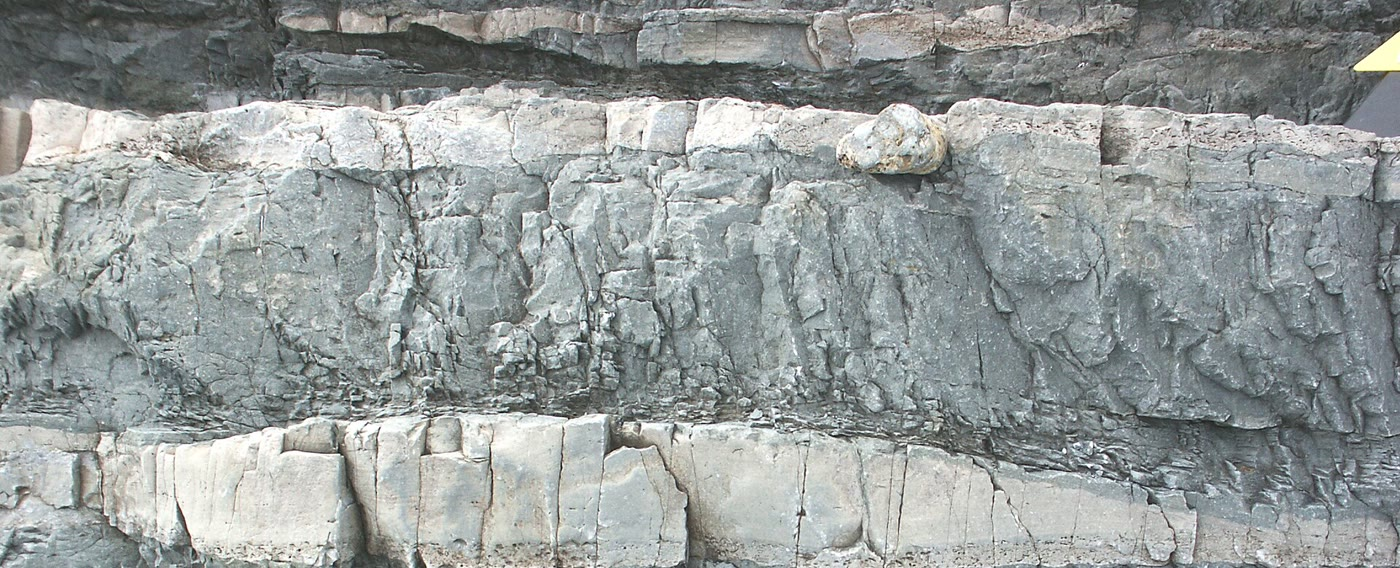
\includegraphics[width=\linewidth]{images/book5/b3-hummocky-cross-stratification.jpg}

{\scriptsize \omterm{def:b3:facies-models:hcs}{Stratifikasi silang hummocky} di Formasi Arisaig
(Silur), dekat Arisaig, Nova Scotia. Foto Michael C. Rygel, CC BY-SA 3.0
(dipotong).}
\end{minipage}
\end{inthefield}
% ledger: photo:b3-hcs

Di tempat pasang surut mendominasi, fasiesnya berubah: arus pasang dan arus surut membentuk
perlapisan silang yang menghadap ke arah berlawanan, endapan lumpur tipis mengendap pada setiap air diam,
dan ketebalan berkas di antara endapan lumpur tersebut membesar dan mengecil mengikuti
siklus pasang perbani dan pasang mati. Saluran pasang surut, dataran, dan punggung pasir
memiliki model sendiri, dibangun dengan cara yang sama.

\section{Laut dalam}\label{sec:b3:facies-models:deep}

Arus turbidit yang melambat mengendapkan muatannya sesuai urutan pengendapan:
butir paling kasar lebih dulu, yang paling halus terakhir. Lapisan turbidit yang lengkap menunjukkan
urutan ini dalam lima divisi.

\begin{definition}[Sekuen Bouma]\label{def:b3:facies-models:bouma}
Yang disebut \emph{sekuen Bouma}\index{sekuen Bouma} adalah suksesi ideal
divisi dalam lapisan turbidit, dari dasar ke atas: Ta, pasir masif atau bergradasi di atas
dasar erosional dengan tanda alur dan tanda perkakas; Tb, pasir berlaminasi sejajar; Tc,
pasir halus berlaminasi riak dan terlipat-lipat; Td, lanau berlaminasi sejajar;
Te, lumpur, sebagian berasal dari arus turbidit dan sebagian dari pengendapan lambat
di antara aliran.
\end{definition}

Sedikit lapisan yang menunjukkan kelima divisi: dekat sumber arusnya cepat dan meninggalkan divisi Ta yang tebal,
dengan bagian atasnya tererosi oleh aliran berikutnya; jauh dari sumber hanya
divisi yang lebih halus, Tc sampai Te, yang tiba. Dengan demikian, sekuen ini merekam
melemahnya satu aliran, dan perubahan lapisan sepanjang kipas merekam melemahnya
aliran seiring jarak.

\begin{definition}[Kipas bawah laut]\label{def:b3:facies-models:fan}
Yang disebut \emph{kipas bawah laut}\index{kipas bawah laut} adalah kerucut sedimen di kaki
lereng benua, yang diumpankan oleh sebuah ngarai: kipas atas dengan alur utama
di antara tanggul alam, kipas tengah berupa saluran distributari yang berakhir di lobus pasir,
dan kipas bawah berupa turbidit tipis yang beralih menjadi lumpur dasar cekungan.
\end{definition}

Di sepanjang tepi benua, arus laut dalam yang digerakkan oleh sirkulasi samudra mengolah
sedimen halus lereng menjadi kontourit, gundukan, dan drift
lanau dan lumpur terbioturbasi yang tumbuh sepanjang kontur, bukan turun
menuruni lereng.

\begin{omfigure}
\begin{tikzpicture}[font=\scriptsize, x=1cm, y=1cm]
% (a) Bouma log
\begin{scope}
\fill[yellow!45] (0,0) -- (1.6,0) -- (1.6,1.2) -- (0,1.2) -- cycle;
\fill[yellow!35] (0,1.2) rectangle (1.3,1.8);
\fill[yellow!25] (0,1.8) rectangle (1.0,2.4);
\fill[black!12] (0,2.4) rectangle (0.7,2.8);
\fill[black!25] (0,2.8) rectangle (0.4,3.3);
\draw (0,0) -- (1.6,0) -- (1.6,1.2) -- (1.3,1.2) -- (1.3,1.8) -- (1.0,1.8) -- (1.0,2.4) -- (0.7,2.4) -- (0.7,2.8) -- (0.4,2.8) -- (0.4,3.3) -- (0,3.3) -- cycle;
\draw[decorate, decoration={snake, amplitude=0.5mm, segment length=2mm}] (0,0) -- (1.6,0);
\foreach \y in {1.35,1.5,1.65} {\draw[black!60] (0.05,\y) -- (1.25,\y);}
\foreach \x in {0.15,0.45,0.75} {\draw[black!60] (\x,1.95) .. controls (\x+0.08,2.1) .. (\x+0.2,1.95);}
\foreach \y in {2.5,2.6,2.7} {\draw[black!60] (0.05,\y) -- (0.65,\y);}
\foreach \y/\t in {0.6/Ta, 1.5/Tb, 2.1/Tc, 2.6/Td, 3.05/Te} {\node[anchor=west] at (1.9,\y) {\t};}
\node[anchor=west, align=left, font=\tiny] at (2.4,0.6) {pasir bergradasi atau masif,\\ dasar erosional};
\node[anchor=west, font=\tiny] at (2.4,1.5) {laminae sejajar};
\node[anchor=west, font=\tiny] at (2.4,2.1) {riak, laminae terlipat-lipat};
\node[anchor=west, font=\tiny] at (2.4,2.6) {lanau berlaminasi};
\node[anchor=west, font=\tiny] at (2.4,3.05) {lumpur};
\node[anchor=north] at (1.6,-0.15) {(a) sebuah lapisan turbidit};
\end{scope}
% (b) fan plan
\begin{scope}[xshift=8.2cm, yshift=0.2cm]
\fill[black!8] (-1.0,-0.2) rectangle (5.6,3.1);
\fill[yellow!20] (0.3,2.9) .. controls (1.6,2.6) and (4.9,2.0) .. (5.2,0.9) .. controls (4.6,-0.1) and (1.2,0.1) .. (0.3,1.6) -- cycle;
\fill[yellow!45] (1.9,1.9) ellipse (0.55 and 0.3);
\fill[yellow!45] (2.6,1.0) ellipse (0.55 and 0.3);
\fill[yellow!45] (3.4,1.75) ellipse (0.5 and 0.28);
\draw[omDef, line width=1.4pt] (-0.9,3.0) .. controls (-0.3,2.8) and (0.4,2.6) .. (1.0,2.2);
\draw[omDef, line width=0.8pt] (1.0,2.2) -- (1.6,1.95);
\draw[omDef, line width=0.8pt] (1.0,2.2) -- (2.3,1.15);
\draw[omDef, line width=0.8pt] (1.0,2.2) .. controls (2.0,2.4) .. (3.1,1.85);
\node[anchor=south west] at (-0.95,3.0) {ngarai};
\node[anchor=east] at (0.55,2.0) {tanggul alam};
\node[align=center, font=\tiny] at (2.6,1.0) {lobus};
\node at (4.4,0.7) {kipas bawah};
\node[black!60] at (4.9,2.85) {dasar cekungan};
\node[anchor=north] at (2.3,-0.25) {(b) sebuah kipas bawah laut dalam denah};
\end{scope}
\end{tikzpicture}

\par\smallskip{\small (a) \omterm{def:b3:facies-models:bouma}{Sekuen Bouma} dari lapisan turbidit lengkap,
digambar sebagai log ukuran butir (lebar berarti lebih kasar), dengan kelima bagiannya. (b)
\omterm{def:b3:facies-models:fan}{Kipas bawah laut} dalam denah: sebuah ngarai memasok alur di antara tanggul alam,
yang bercabang menjadi alur distributari yang berakhir pada lobus pasir; turbidit tipis
menyebar di atas bagian bawah kipas.}\label{fig:b3:facies-models:deep}
\end{omfigure}

\section{Platform karbonat}\label{sec:b3:facies-models:carbonates}

Sedimen karbonat terbentuk di tempat ia berada, oleh organisme di perairan dangkal yang hangat dan jernih,
dan fasiesnya mengikuti profil platform yang
dibangun oleh pabrik karbonat untuk dirinya sendiri.

\begin{definition}[Landaian karbonat dan paparan bertepi]\label{def:b3:facies-models:ramp}
Yang disebut \emph{landaian karbonat}\index{landaian karbonat} adalah platform yang dasarnya
miring landai dan merata dari garis pantai ke cekungan, tanpa putus:
sabuk fasiesnya, dari dataran pasang surut dan pasir penghalang gisik hingga butir gosong,
pasir bioklastik, dan lumpur kapur lepas pantai, lebar dan berangsur menyatu satu sama lain,
tersortir oleh energi gelombang yang menurun seiring kedalaman. Sebuah \emph{paparan
bertepi}\index{paparan bertepi} adalah platform berpuncak datar dengan patahan kemiringan yang jelas di
tepinya, tempat terumbu dan gosong pasir membentuk tepi yang melindungi
laguna di belakangnya; di luar tepi, lereng curam melepaskan blok dan butir ke dalam
cekungan.
\end{definition}

\begin{omfigure}
\begin{tikzpicture}[font=\scriptsize, x=1cm, y=1cm]
\begin{scope}
\fill[omSea!60] (0,1.6) -- (6.4,1.6) -- (6.4,0.3) -- cycle;
\fill[black!10] (0,1.6) -- (6.4,0.3) -- (6.4,0) -- (0,0) -- cycle;
\draw[thick] (0,1.7) -- (0.3,1.6) -- (6.4,0.3);
\draw[omDef] (0,1.6) -- (6.4,1.6);
\node[anchor=south] at (0.6,1.65) {dataran pasang surut};
\node[rotate=-12, font=\tiny] at (1.5,1.08) {butir gosong};
\node[rotate=-12, font=\tiny] at (3.4,0.66) {pasir bioklastik};
\node[rotate=-12, font=\tiny] at (5.3,0.26) {lumpur kapur};
\node[anchor=north] at (3.2,-0.1) {(a) landaian: lereng landai, sabuk bertahap};
\end{scope}
\begin{scope}[xshift=7.2cm]
\fill[omSea!60] (0,1.6) -- (6.4,1.6) -- (6.4,0.2) -- (4.4,0.3) -- (3.6,1.55) -- (3.2,1.6) -- (0.3,1.6) -- cycle;
\fill[omSea!60] (0.3,1.6) -- (3.2,1.6) -- (3.0,1.35) -- (0.6,1.35) -- cycle;
\fill[black!10] (0,1.7) -- (0.3,1.6) -- (0.6,1.35) -- (3.0,1.35) -- (3.2,1.6) -- (3.6,1.55) -- (4.4,0.3) -- (6.4,0.2) -- (6.4,0) -- (0,0) -- cycle;
\draw[thick] (0,1.7) -- (0.3,1.6) -- (0.6,1.35) -- (3.0,1.35) -- (3.2,1.6) -- (3.6,1.55) -- (4.4,0.3) -- (6.4,0.2);
\fill[orange!50] (3.05,1.4) -- (3.2,1.6) -- (3.55,1.56) -- (3.6,1.4) -- cycle;
\draw[omDef] (0,1.6) -- (6.4,1.6);
\node at (1.8,1.12) {laguna};
\node[anchor=south] at (3.35,1.65) {tepi terumbu};
\node[anchor=west] at (4.2,0.95) {lereng curam};
\node at (5.5,0.6) {cekungan};
\node[anchor=north] at (3.2,-0.1) {(b) paparan bertepi: tepi, laguna, lereng};
\end{scope}
\end{tikzpicture}

\par\smallskip{\small Profil platform karbonat (skematis, skala vertikal
sangat diperbesar). (a) Landaian: sabuk tersortir oleh energi gelombang di sepanjang
lereng landai. (b) \omterm{def:b3:facies-models:ramp}{Paparan bertepi}: terumbu dan tepi gosong di titik patahan kemiringan
melindungi laguna lumpur kapur; lereng di belakangnya menerima blok dan butir
yang lepas dari tepi.}\label{fig:b3:facies-models:platforms}
\end{omfigure}

Pada permukaan platform yang datar, sedikit kenaikan muka laut relatif menggenangi dataran
pasang surut, dan pabrik, yang bekerja paling cepat di perairan terdangkal, mengisi
kembali ruang itu sampai ke muka laut dalam waktu singkat. Hasilnya adalah tumpukan
siklus peritidal setebal satu meter atau beberapa meter, masing-masing berupa
\omterm{def:b3:sequence-stratigraphy:parasequence}{parasekuen} menyusut ke atas dari lumpur subtidal hingga dataran pasang surut dengan retakan
pengeringan atau hamparan mikroba, ditutup oleh \omterm{def:b3:sequence-stratigraphy:parasequence}{permukaan genang} berikutnya.

\section{Inti dan log sumur}\label{sec:b3:facies-models:logs}

Sebagian besar batuan di bawah cekungan sedimen diketahui dari lubang bor. Sebagian kecil
diambil intinya, dan intinya dideskripsikan lapisan demi lapisan seperti tebing; hampir semua
dicatat log-nya.

\begin{definition}[Log kabel]\label{def:b3:facies-models:wireline}
Sebuah \emph{log kabel}\index{log kabel} adalah rekaman kontinu tentang
suatu sifat fisis batuan terhadap kedalaman, diukur oleh probe yang diturunkan
dengan kabel ke dalam lubang bor. \emph{Log sinar gamma}\index{log sinar gamma}
mencatat radiasi gamma alami batuan, dalam satuan API: tinggi pada
serpih, yang lempungnya menyimpan kalium, torium, dan uranium, rendah pada pasir kuarsa bersih
dan pada batu gamping. \emph{Log densitas}\index{log densitas}
mencatat massa jenis total dari hamburan sinar gamma yang dipancarkan oleh
sumber pada probe. \emph{Log sonik}\index{log sonik} mencatat
waktu tempuh interval gelombang kompresional, dalam mikrodetik per kaki.
\emph{Log neutron}\index{log neutron} mencatat perlambatan neutron oleh hidrogen,
dan karena itu air yang tersimpan di dalam pori dan di dalam lempung.
\end{definition}
% ledger: keys:gamma, keys:density-porosity, keys:sonic

Satuan radiasi gamma API didefinisikan di kolam kalibrasi: satu per dua ratus dari
selisih antara zona dengan radioaktivitas yang dapat diabaikan dan zona dengan
radioisotop serpih rata-rata pada sekitar dua kali konsentrasinya. Batu bara,
batu gamping, dan dolomit biasanya kurang radioaktif dibanding serpih; batu pasir
kuarsa rendah, arkosa yang kaya feldspar kalium lebih tinggi; batuan apa pun dapat
menjadi radioaktif oleh uranium yang dibawa air tanah.
% ledger: keys:gamma

\begin{proposition}[Porositas dari massa jenis dan waktu tempuh]\label{prop:b3:facies-models:porosity}
Batuan dengan porositas $\phi$, dengan butir dengan massa jenis $\rho_{\mathrm{ma}}$ dan
pori yang terisi fluida dengan massa jenis $\rho_f$, memiliki massa jenis total
$\rho_b = (1 - \phi)\rho_{\mathrm{ma}} + \phi\rho_f$, sehingga
\[
\phi = \frac{\rho_{\mathrm{ma}} - \rho_b}{\rho_{\mathrm{ma}} - \rho_f}.
\]
Jika gelombang kompresional melewati butir dan fluida secara seri, dengan
panjang yang sebanding dengan $1 - \phi$ dan $\phi$, waktu tempuhnya
$\Delta t = (1 - \phi)\Delta t_{\mathrm{ma}} + \phi\Delta t_f$ (persamaan
rata-rata waktu), dan $\phi = (\Delta t - \Delta
t_{\mathrm{ma}})/(\Delta t_f - \Delta t_{\mathrm{ma}})$.
\end{proposition}

\begin{proof}
Sebuah satuan volume batuan memuat volume $1 - \phi$ butiran dan $\phi$
fluida; massanya $(1 - \phi)\rho_{\mathrm{ma}} + \phi\rho_f$, yang kemudian diselesaikan
untuk $\phi$. Untuk gelombang, lintasan sepanjang satu satuan memotong $1 - \phi$ butiran
dan $\phi$ fluida, dan waktu tempuhnya dijumlahkan.
\end{proof}

Massa jenis butiran adalah \qty{2.65}{g/cm^3} untuk kuarsa dan \qty{2.71}{g/cm^3} untuk batu gamping;
air pori adalah \qty{1.0}{g/cm^3} saat tawar dan hingga
\qty{1.1}{g/cm^3} sebagai air garam. Waktu tempuh berkisar dari 42 hingga
\qty{48}{\micro\second/ft} pada dolomit, 48 hingga 53 pada batu gamping, 53 untuk batu pasir
terkonsolidasi, dan 189 pada air garam. Persamaan massa jenis bersifat eksak untuk
matriks yang diketahui; persamaan rata-rata waktu adalah aturan empiris yang paling baik
bekerja pada batuan terkonsolidasi dengan pori antarbutir. Serpih melanggar keduanya:
lempung memiliki massa jenisnya sendiri dan menahan air terikat.
% ledger: keys:density-porosity, keys:sonic

\begin{definition}[Rasio neto terhadap bruto]\label{def:b3:facies-models:ntg}
Yang disebut \emph{rasio neto terhadap bruto}\index{rasio neto terhadap bruto} suatu interval adalah
ketebalan batuan berkualitas reservoir, biasanya pasir yang diidentifikasi pada \omterm{def:b3:facies-models:wireline}{log sinar gamma}
di bawah suatu batas potong, dibagi dengan ketebalan total interval tersebut.
\end{definition}

Bentuk kurva sinar gamma melalui suatu tubuh pasir merupakan alat fasies.
Bentuk \emph{lonceng}, bersih di dasar dan makin serpih ke atas, merupakan
\omterm{def:b3:facies-models:association}{suksesi menghalus ke atas}, seperti pada \omterm{def:b3:facies-models:rivers}{gosong tepi} atau isian alur; bentuk \emph{corong}, serpih di
dasar dan bersih di atas, merupakan \omterm{def:b3:facies-models:association}{suksesi mengasar ke atas}, seperti pada
\omterm{def:b3:facies-models:shoreface}{muka pantai} progradasi atau front delta; bentuk \emph{silinder}, bersih di seluruh bagian dengan
batas tajam, menunjukkan pasir \omterm{def:b3:facies-models:rivers}{sungai teranyam} bertumpuk, gumuk pasir eolian, atau
gosong karbonat. Bentuk-bentuk ini hanyalah petunjuk, bukan bukti: sebuah inti, atau setidaknya
log tetangga, harus mengonfirmasinya.

\begin{omfigure}
\begin{tikzpicture}
\begin{groupplot}[group style={group size=3 by 1, horizontal sep=0.2cm,
    y descriptions at=edge left},
  omrecord, y dir=reverse, ymin=700, ymax=1200, width=0.28\linewidth,
  height=0.62\linewidth, ytick={700,800,900,1000,1100,1200},
  tick label style={font=\scriptsize}, label style={font=\small},
  xlabel style={font=\small}]
\nextgroupplot[xlabel={GR (API)}, ylabel={kedalaman (m)}, xmin=0, xmax=150,
  xtick={0,50,100,150}]
\addplot[black!60, densely dashed, forget plot] coordinates {(60,1046) (60,1166)};
% computed in figdata/bachelor-3/well_logs.py
\addplot[omDef, thin] table[x=gr, y=depth] {figdata/out/bachelor-3-well_logs-logs.dat};
\node[font=\scriptsize, anchor=west] at (axis cs:2,730) {kapur};
\node[font=\scriptsize, anchor=west] at (axis cs:2,816) {serpih};
\node[font=\scriptsize, anchor=west] at (axis cs:28,956) {batu gamping};
\node[font=\scriptsize, anchor=west] at (axis cs:28,1030) {batu pasir};
\node[font=\scriptsize, anchor=west] at (axis cs:2,1185) {sekis};
\nextgroupplot[xlabel={$\rho_b$ (\unit{g/cm^3})}, xmin=1.9, xmax=2.9,
  xtick={2.0,2.4,2.8}, xticklabels={2.0,2.4,2.8}]
\addplot[red!70!black, thin] table[x=rhob, y=depth] {figdata/out/bachelor-3-well_logs-logs.dat};
\nextgroupplot[xlabel={$\Delta t$ (\unit{\micro\second/ft})}, xmin=40, xmax=140,
  x dir=reverse, xtick={40,80,120}]
\addplot[green!40!black, thin] table[x=dt, y=depth] {figdata/out/bachelor-3-well_logs-logs.dat};
\end{groupplot}
\begin{axis}[at={(group c3r1.south east)}, xshift=1.35cm, anchor=south west,
  omrecord, y dir=reverse, ymin=1040, ymax=1172, width=0.28\linewidth,
  height=0.62\linewidth, xmin=0, xmax=120, xtick={0,60,120},
  ytick={1040,1060,1080,1100,1120,1140,1160}, ylabel={kedalaman (m)},
  xlabel={GR (API), batu pasir}, tick label style={font=\scriptsize},
  label style={font=\small}]
\addplot[black!60, densely dashed, forget plot] coordinates {(60,1046) (60,1166)};
\addplot[omDef, semithick] table[x=gr, y=depth] {figdata/out/bachelor-3-well_logs-sand.dat};
\end{axis}
\end{tikzpicture}

\par\smallskip{\small Log sintetik sumur Varden-2 dari \qty{700}{m}
hingga batuan dasar: sinar gamma (garis putus-putus adalah batas potong pasir
sebesar \qty{60}{API} pada batu pasir), densitas curah dan waktu tempuh sonik (waktu
bertambah ke kiri, seperti log digambar); kanan, sinar gamma batu pasir yang
diperbesar. Kapur menjadi lebih padat dengan kedalaman;
serpih terbaca panas, lambat, dan bermassa jenis menengah; batu gamping dingin,
padat dan cepat; batu pasir merupakan tumpukan isian alur, masing-masing dengan dasar bersih
yang beralih ke atas menjadi lumpur: bentuk lonceng.}\label{fig:b3:facies-models:logs}
\end{omfigure}
% ledger: keys:gamma, keys:density-porosity, keys:sonic

\begin{inthelab}[Membuat log inti]
\begin{minipage}[t]{0.5\linewidth}\vspace{0pt}
Di gudang inti, inti sebuah sumur ditata dalam baki, dibelah
memanjang, sesuai urutan kedalamannya. Seorang sedimentolog mendeskripsikan inti
itu lapisan demi lapisan pada lembar log: ukuran butir dengan lup tangan dan bagan pembanding,
struktur, kontak, fosil, jejak liang dan akar, warna
lumpur. Deskripsi itu kemudian disandingkan dengan \omterm{def:b3:facies-models:wireline}{log kabel} pada
kedalaman yang sama, sehingga bentuk log dapat dikalibrasi terhadap batuan dan
sumur tak berinti di sekitarnya dapat dibaca.
\end{minipage}\hfill
\begin{minipage}[t]{0.46\linewidth}\vspace{0pt}
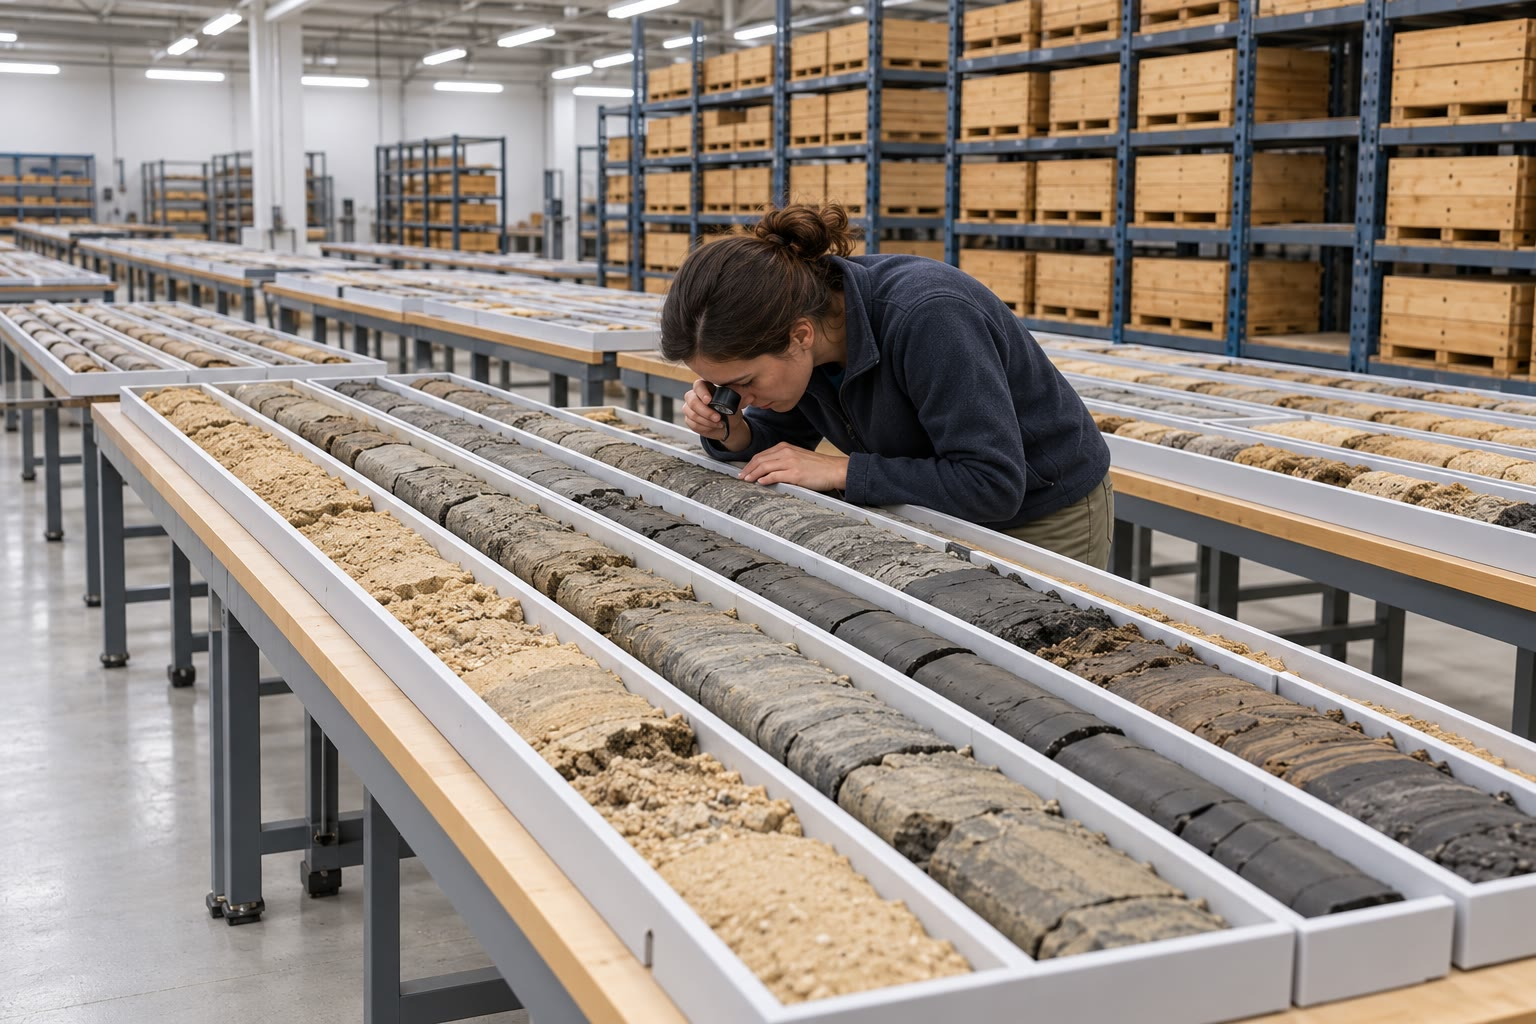
\includegraphics[width=\linewidth]{images/book5/ai/b3-core-store.jpg}

{\scriptsize Gudang inti: inti terbelah berupa pasir dan lumpur dalam baki, seorang ahli geologi
dengan lup tangan. Ilustrasi buatan AI.}
\end{minipage}
\end{inthelab}

\section{Latihan}

\begin{exercise}[$\star$]\label{exo:b3:facies-models:1}
Sebuah inti menunjukkan, dari dasar ke atas: lumpur lepas pantai, lumpur berselang-seling dengan pasir halus,
pasir \omterm{def:b3:facies-models:shoreface}{muka pantai}, pasir gisik, lalu batu bara dengan akar. Dengan menggunakan hukum Walther, berikan
urutan lingkungan sepanjang pesisir pada saat itu dan arah
ke mana garis pantai bergerak. Apa yang akan ditinggalkan oleh transgresi?
\end{exercise}

\begin{exercise}[$\star$]\label{exo:b3:facies-models:2}
Tiga tubuh pasir menunjukkan bentuk sinar gamma: (a) lonceng setebal \qty{8}{m} dengan
dasar tajam; (b) corong setebal \qty{20}{m}; (c) silinder setebal \qty{30}{m}
dengan puncak dan dasar tajam. Usulkan lingkungan untuk masing-masing, dan
pengamatan pada inti yang akan mengonfirmasinya.
\end{exercise}

\begin{exercise}[$\star$]\label{exo:b3:facies-models:3}
Sebuah batu pasir menunjukkan $\rho_b = \qty{2.40}{g/cm^3}$. Hitung porositasnya dengan
matriks kuarsa dan air tawar, lalu dengan air garam \qty{1.1}{g/cm^3}.
\end{exercise}
% ledger: keys:density-porosity

\begin{exercise}[$\star$]\label{exo:b3:facies-models:4}
Gelombang dengan panjang gelombang modal \qty{75}{m} dan \qty{110}{m} (laut terlindung dan
laut terbuka pada studi pelampung). Taksir kedalaman tempat masing-masing
mempertahankan \qty{4}{\percent} dari gerak permukaannya, serta fraksi yang tersisa
pada kedalaman \qty{20}{m}.
\end{exercise}
% ledger: losspeters10:wavebase

\begin{exercise}[$\star\star$]\label{exo:b3:facies-models:5}
Sebuah batu gamping menunjukkan $\Delta t = \qty{60}{\micro\second/ft}$. Hitung
porositasnya dengan persamaan rata-rata waktu untuk matriks dengan nilai 47.6 dan
\qty{52.6}{\micro\second/ft} serta air garam pada \qty{189}{\micro\second/ft}. Apa
yang dapat dipelajari dari selisih tersebut?
\end{exercise}
% ledger: keys:sonic

\begin{exercise}[$\star\star$]\label{exo:b3:facies-models:6}
Interval \qty{40}{m} memuat lapisan pasir dengan ketebalan 6.0, 3.5, 8.0 dan \qty{2.5}{m}
di bawah batas potong, sisanya lumpur. Hitung \omterm{def:b3:facies-models:ntg}{rasio neto terhadap bruto}. Dengan
porositas \qty{22}{\percent} pada pasir, berapa volume pori yang dimiliki satu kilometer
persegi interval tersebut?
\end{exercise}

\begin{exercise}[$\star\star$]\label{exo:b3:facies-models:7}
Lapisan turbidit dekat mulut ngarai berupa \qty{1.2}{m} pasir masif (Ta) yang tererosi di
bagian atasnya oleh lapisan berikutnya; sejauh \qty{30}{km} ke bawah kipas, lapisan
dari aliran yang sama berupa \qty{8}{cm} pasir halus dan lanau berlaminasi riak di bawah
\qty{3}{cm} lumpur. Sebutkan divisi masing-masing dan jelaskan perubahannya.
\end{exercise}

\begin{exercise}[$\star\star$]\label{exo:b3:facies-models:8}
\omterm{def:b3:facies-models:association}{Suksesi menghalus ke atas} setebal \qty{9}{m} memiliki dasar tajam dengan kerakal,
pasir bersilang, pasir halus berlaminasi riak dan lumpur berakar. Interpretasikan, dan
taksirlah kedalaman alur yang membentuknya. Dapatkah hukum Walther
diterapkan lintas dasarnya? Mengapa?
\end{exercise}

\begin{exercise}[$\star\star$]\label{exo:b3:facies-models:9}
Dasar sebuah platform turun \qty{60}{m} sepanjang \qty{40}{km}; platform lain
mempertahankan kedalaman \qty{5}{m} selama \qty{30}{km}, lalu turun \qty{300}{m} sepanjang
\qty{1.5}{km}. Hitung kedua gradien, sebutkan setiap platform dan fasies yang
diharapkan di tepi yang kedua.
\end{exercise}

\begin{exercise}[$\star\star\star$]\label{exo:b3:facies-models:10}
Garis pantai berprogradasi dengan kecepatan $v$ sementara muka laut relatif naik dengan laju
$A$, dan sabuk \omterm{def:b3:facies-models:shoreface}{muka pantainya} selebar $w$. Tunjukkan bahwa pasir \omterm{def:b3:facies-models:shoreface}{muka pantai} dalam
suksesi vertikal memiliki ketebalan $h = wA/v$. Hitung untuk $w = \qty{2}{km}$,
$A = \qty{0.2}{m/ka}$ dan $v = \qty{20}{m/ka}$, lalu nyatakan apa yang terjadi ketika
$A = 0$. Bandingkan dengan proposisi tentang \omterm{def:b3:sequence-stratigraphy:trajectory}{lintasan garis pantai} di
Bab~\ref{ch:b3:sequence-stratigraphy}.
\end{exercise}

\begin{exercise}[$\star\star\star$]\label{exo:b3:facies-models:11}
Sebuah batu pasir menunjukkan $\rho_b = \qty{2.30}{g/cm^3}$ dan $\Delta t =
\qty{86}{\micro\second/ft}$. Hitung porositasnya dari masing-masing log dengan matriks
batu pasir kuarsa (2.65, \qty{52.6}{\micro\second/ft}) dan air garam (1.0 untuk
massa jenis, \qty{189}{\micro\second/ft}). Jika porositas sonik benar, massa jenis butir
apa yang disiratkan \omterm{def:b3:facies-models:wireline}{log densitas}, dan apa kemungkinan semennya?
\end{exercise}
% ledger: keys:density-porosity, keys:sonic

\begin{exercise}[$\star\star\star$]\label{exo:b3:facies-models:12}
Dalam sebuah inti, lumpur lepas pantai hitam langsung berada di atas batu bara berakar, dengan
lapisan tipis pecahan cangkang di kontaknya. Jelaskan mengapa hukum Walther tidak
berlaku lintasnya, apa jenis permukaannya, dan berapa banyak suksesi pesisir
mungkin hilang jika gelombang mengikis dasar sampai \omterm{def:b3:facies-models:shoreface}{dasar gelombang cuaca cerah}
sekitar \qty{10}{m} saat garis pantai bergeser.
\end{exercise}

\section{Soal: Varden-2, sumur melalui penutup}

\begin{problem}[{Soal akhir pekan --- log, porositas, fasies dan pasir neto
sebuah sumur rekaan di sinklin Varden}]
\label{pb:b3:facies-models:1}
Sumur Varden-2 dibor di sinklin Bukit Varden, pada
(7500, 7000) pada kisi wilayah, dari elevasi permukaan tanah
\qty{441.0}{m}, hingga kedalaman total \qty{1200}{m}. Log-nya tergambar pada
gambar di bagian terakhir. Gunakan massa jenis butir 2.65 (kuarsa) dan
\qty{2.71}{g/cm^3} (kalsit), air pori \qty{1.0}{g/cm^3}, waktu transit matriks
52.6 (batu pasir) dan \qty{47.6}{\micro\second/ft}
(batu gamping), serta \qty{189}{\micro\second/ft} untuk air.

\medskip\noindent\textbf{Bagian I --- Membaca log.}
\begin{enumerate}
\item Sinar gamma melonjak dari 12 ke \qty{110}{API} pada \qty{766}{m}, turun
  ke 18 pada \qty{866}{m}, menjadi tidak teratur dari \qty{1046}{m} dan stabil pada
  \qty{85}{API} dari \qty{1166}{m}. Sebutkan unit yang dijumpai, dengan memakai log-nya.
\item Hitung ketebalan setiap unit penutup dan elevasi
  dasar penutup.
\item Kapur menunjukkan \qty{2.03}{g/cm^3} dekat permukaan dan
  \qty{2.36}{g/cm^3} pada \qty{750}{m}. Hitung porositasnya pada kedua kedalaman.
  Apa yang terjadi pada kapur seiring kedalaman?
\item Mengapa serpih tidak diberi porositas dari massa jenisnya?
\item Sekis menunjukkan \qty{2.75}{g/cm^3} dan \qty{50}{\micro\second/ft}.
  Apa yang dikatakan basemen yang cepat, padat dan tidak berpori kepada pengebor?
\end{enumerate}

\medskip\noindent\textbf{Bagian II --- Porositas.}
\begin{enumerate}[resume]
\item Batu gamping menunjukkan \qty{2.573}{g/cm^3}: hitung porositas densitasnya.
\item Ia menunjukkan \qty{58.9}{\micro\second/ft}: hitung porositas sonik dan
  bandingkan.
\item Pasir bersih pada isian alur menunjukkan \qty{2.32}{g/cm^3}: hitung
  porositasnya.
\item Periksa dengan waktu transitnya, \qty{79.9}{\micro\second/ft}.
\item Jika air pori berupa air garam \qty{1.1}{g/cm^3}, seberapa besar
  porositas densitas pasir akan berubah?
\item Unit mana yang lebih baik sebagai akuifer atau reservoir, dan
  mana penyekat di atasnya?
\end{enumerate}

\medskip\noindent\textbf{Bagian III --- Fasies.} Inti yang diambil dari 1108 sampai
\qty{1124}{m} menunjukkan, dari dasar: permukaan tergerus dengan fragmen lumpur dan
kerakal; \qty{10.4}{m} pasir sedang berlapis silang; \qty{3.2}{m} pasir
halus berriak yang beralih menjadi lanau; \qty{2.4}{m} lumpur cokelat-merah dengan jejak akar.
\begin{enumerate}[resume]
\item Gambarkan bentuk sinar gamma yang diharapkan sepanjang interval inti yang diambil.
\item Tentukan suksesi dan lingkungan pengendapan setiap bagian.
\item Dengan hukum Walther, jelaskan lingkungan yang terletak berdampingan.
\item Buat taksiran kedalaman alur.
\item Batu pasir ini memuat sebelas unit semacam itu, masing-masing dengan dasar tajam. Apa
  yang diungkapkan penumpukannya tentang sungai dan dataran banjirnya?
\item Dapatkah hukum Walther digunakan untuk berpindah dari satu unit ke unit berikutnya? Mengapa?
\end{enumerate}

\medskip\noindent\textbf{Bagian IV --- Pasir neto.} Sebelas isian alur,
dari dasar batu pasir, berturut-turut setebal 14, 9, 12, 7, 16, 10, 13, 8, 11, 12 dan
\qty{8}{m}. Tiap unit dimulai dengan pasir bersih (\qty{30}{API}) yang menempati
sebagian dari ketebalannya, yakni 0.60, 0.45, 0.55, 0.30, 0.65, 0.40, 0.55, 0.35, 0.50,
0.45 dan 0.30, lalu menghalus ke atas pada bagian sebesar 0.25, 0.30, 0.25, 0.40,
0.20, 0.30, 0.25, 0.35, 0.25, 0.30 dan 0.35, dengan sinar gamma naik secara linear hingga
\qty{105}{API}, dan diakhiri dengan lumpur.
\begin{enumerate}[resume]
\item Berapa bagian dari tiap interval penghalusan yang berada di bawah
  batas potong \qty{60}{API}?
\item Hitung pasir neto unit terbawah dan unit yang paling tebal.
\item Hitung total pasir bersih dan total interval penghalusan dari
  batu pasir tersebut.
\item Hitung \omterm{def:b3:facies-models:ntg}{rasio neto terhadap brutonya}.
\item Bagaimana pasir neto akan berubah dengan batas potong 45 atau
  \qty{75}{API}?
\item Dengan porositas pasir pada pertanyaan 8, hitung volume pori dari pasir neto
  di bawah satu kilometer persegi.
\item Nyatakan tebal pasir neto dari batu pasir Trias di Varden-2.
\end{enumerate}
\end{problem}
% ledger: keys:density-porosity, keys:sonic, keys:gamma
